% Condensed LaTeX version of Kuo (1998), J. Biomech. Eng. 120:148-159.
% Prose is condensed; all equations are reproduced, with printed errors
% corrected in place and flagged by "Transcription note" footnotes.
\documentclass[11pt]{article}
\usepackage[margin=1in]{geometry}
\usepackage{amsmath,amssymb}
\usepackage{siunitx}
\usepackage{tikz}
\usetikzlibrary{arrows.meta}

\newcommand{\tnote}[1]{\footnote{\textit{Transcription note.} #1}}

\title{A Least-Squares Estimation Approach to Improving the Precision of
Inverse Dynamics Computations}
\author{A. D. Kuo\\[2pt]
\small Department of Mechanical Engineering \& Applied Mechanics\\
\small University of Michigan, Ann Arbor, MI 48109}
\date{\small Condensed transcription of \cite{Kuo1998}}

\begin{document}
\maketitle

\noindent\fbox{\parbox{\dimexpr\textwidth-2\fboxsep-2\fboxrule}{\small
\textbf{About this document.} This is a condensed LaTeX version of
\cite{Kuo1998}, prepared as a working reference for the equations. The prose
is summarized, not reproduced; consult the original article for its exact
wording, and for Figs.~2--7, which are not reproduced here. All equations
and equation numbers follow the original; matrix products are written by
juxtaposition, where the original uses a centered dot. Where the original contains a
typographical or sign error, the corrected equation is shown and a
\emph{Transcription note} footnote records what was printed. The
corrected equations of Appendix~A were checked numerically against a
direct segment-by-segment Newton--Euler computation of the four-segment
model.}}

\begin{abstract}
The paper computes inverse dynamics by least squares. The equations of motion
of a multi-segment body are augmented with terms for the ground reaction
forces and torque. Kinematic and force measurements then outnumber the
unknown joint torques at every instant, so the system is overdetermined; it is
solved by weighted least squares for the joint torques and angular
accelerations that best agree with the measurements. Estimation theory gives
predicted error magnitudes for both the conventional Newton--Euler method and
the least-squares method. A variant of the method also removes constant
biases, such as those caused by misalignment between force plate and motion
capture reference frames. In a simulated benchmark, joint torque errors fall
by about 30 percent relative to Newton--Euler over a wide range of noise
levels. The method uses all available measurements, works with an incomplete
set of ground reaction measurements, produces no residual torque on the
top-most segment, and can reject constant biases.
\end{abstract}

\section*{Introduction}

Inverse dynamics estimates joint torques (moments of muscle force) from
motion data, and is a standard tool for analyzing gait and other movements. It
needs anthropometric parameters, limb kinematics, and often ground reaction
forces, all of which are measured imperfectly, so it is worth extracting the
most precise torque estimates possible from them.

The conventional approach \cite{Winter1990} iterates the Newton--Euler
equations segment by segment, starting at the top-most segment. Because
angular accelerations come from twice-differentiated position data, which
amplifies noise, the resulting torques are noisy. Ground reaction forces can
be used as boundary conditions at the bottom-most segment instead, and are
usually more precise, but they add more equilibrium conditions than can be
satisfied. The excess is usually absorbed either by discarding accelerations
at the top-most segment or by allowing residual forces and torques there.

Two optimization-based alternatives exist. Vaughan et al.\
\cite{VaughanEtAl1982} used the extra degrees of freedom introduced by ground
reaction forces to optimize the body segment parameters; this improves those
parameters but does not otherwise change the torque estimates. Dynamic
optimization \cite{ChaoRim1973} finds the joint torque trajectory whose
forward simulation best reproduces the measured motion. It enforces the
dynamics over time and is the theoretically ideal method, but it is hard to
initialize and expensive to solve, because a standing or walking human is
unstable and simulations diverge from all but very good initial guesses.
Both conventional and dynamic methods are also sensitive to errors such as
mismatched force-plate and motion-capture origins \cite{McCawDeVita1995}.

This paper instead treats inverse dynamics as an overcomplete system of
equations solved by static optimization at each instant. It is less precise
than dynamic optimization in principle, but much easier and faster, and
compared with the conventional method it (i) uses all available data,
rejecting random noise; (ii) gives torques consistent with the equations of
motion, with no residual forces or torques; (iii) works without a full set of
ground reaction measurements; and (iv) can be extended to remove biases from
reference-frame mismatch. Parts of the work appeared earlier
\cite{Kuo1994,Kuo1995}. The paper presents the method, predicts the errors of
both methods by estimation theory, tests them on a simulated postural task
with known torques, and adds a formulation for eliminating measurement bias.

\section*{Nomenclature}

\begin{center}\small
\begin{minipage}[t]{0.48\textwidth}
\begin{tabular}[t]{@{}r@{${}={}$}p{0.6\linewidth}@{}}
$n$ & number of body segments\\
$N$ & number of time steps\\
$\bar{x}_{ci}$ & actual position of segment $i$'s center of mass\\
$x_{ci}$, $x_{ci}'$ & estimated and measured values of $\bar{x}_{ci}$\\
$\dot{\bar{x}}_{ci}$, $\dot{x}_{ci}$, $\dot{x}_{ci}'$ & actual, estimated,
and measured linear velocity\\
$\ddot{\bar{x}}_{ci}$, $\ddot{x}_{ci}$, $\ddot{x}_{ci}'$ & actual, estimated,
and measured linear acceleration\\
$\bar{\phi}_i$ & actual angular orientation (segment angle) of segment $i$\\
$\phi_i$, $\phi_i'$ & estimated and measured values of $\bar{\phi}_i$\\
$\dot{\bar{\phi}}_i$, $\dot{\phi}_i$, $\dot{\phi}_i'$ & actual, estimated, and
measured angular velocity
\end{tabular}
\end{minipage}\hfill
\begin{minipage}[t]{0.48\textwidth}
\begin{tabular}[t]{@{}r@{${}={}$}p{0.6\linewidth}@{}}
$\ddot{\bar{\phi}}_i$, $\ddot{\phi}_i$, $\ddot{\phi}_i'$ & actual, estimated,
and measured angular acceleration\\
$\bar{f}_{i-1}$ & intersegmental reaction force on segment $i$ at joint $i-1$\\
$f_i$, $f_i'$ & estimated and measured values of $\bar{f}_i$\\
$\bar{\tau}_{i-1}$ & actual joint torque (moment of muscle force) on segment
$i$ at joint $i-1$\\
$\tau_i$, $\tau_i'$ & estimated and measured values of $\bar{\tau}_i$\\
$f_0$, $\tau_0$ & estimated ground reaction forces and torque\\
$w_{f0}$, $w_{\tau0}$, $w_{\phi}$ & measurement noise in $f_0'$, $\tau_0'$,
$\phi'$
\end{tabular}
\end{minipage}
\end{center}

\section*{Method}

Rather than treating each segment separately, the method writes the equations
of motion in generalized coordinates for all segments at once. One set of
equations relates joint torques to angular accelerations, with no
intersegmental forces; a second relates joint torques to the ground reaction
forces. Both are linear in the joint torques, and together they form an
overcomplete system that is solved by a weighted pseudoinverse. A stochastic
formulation accounts for measurement noise and predicts the error covariance.
The derivation is for a two-dimensional system; Appendix~C gives the changes
for three dimensions.

\paragraph{Model and notation.} The body has $n$ segments (Fig.~\ref{fig:1}),
numbered $i=1,2,\ldots,n$ from the segment in static contact with the force
plate (typically the foot, assumed motionless) to the most distal. Segment $i$
has center-of-mass position $x_{ci}$ (two components) and orientation
$\phi_i$; the $\phi_i$ fully determine the configuration and serve as
generalized coordinates \cite{Greenwood1988}. Joint $i$, for
$i=1,\ldots,n-1$, connects segments $i$ and $i+1$. On segment $i$, the
intersegmental force $f_{i-1}$ and joint torque $\tau_{i-1}$ act at the end
at joint $i-1$, and $-f_i$ and $-\tau_i$ act at the end at joint $i$. The
ground reaction forces and torque are $f_0$ and $\tau_0$, so the force plate
can be regarded as segment $i=0$. The following quantities are stacked:
\[
\phi \equiv \begin{bmatrix}\phi_2\\ \phi_3\\ \vdots\\ \phi_n\end{bmatrix},
\qquad
\tau \equiv \begin{bmatrix}\tau_1\\ \tau_2\\ \vdots\\ \tau_{n-1}\end{bmatrix}.
\]
An overbar denotes an actual value ($\bar{z}$), a prime a measured value
($z'$), and the unadorned symbol an estimate ($z$). Measurement errors are
additive:
\[
\phi' = \bar{\phi} + w_{\phi}, \qquad
f_0' = \bar{f}_0 + w_{f0}, \qquad
\tau_0' = \bar{\tau}_0 + w_{\tau0},
\]
where $w_{\phi}$, $w_{f0}$, and $w_{\tau0}$ are zero-mean Gaussian white noise
vectors. Angular accelerations are obtained by differentiating the angles
twice,
\[
\ddot{\phi}' = \ddot{\bar{\phi}} + w_{\ddot{\phi}},
\]
where $w_{\ddot{\phi}}$ is (nonwhite) acceleration noise. Since
differentiation amplifies noise, angle and velocity errors are small relative
to acceleration errors, and the estimates are set to the measurements:
$\phi=\phi'$ and $\dot{\phi}=\dot{\phi}'$ ($\phi_1$ is assumed constant).

\paragraph{Conventional Newton--Euler Method.} Newton's and Euler's equations
are applied to each segment at every instant:\tnote{The original prints (1)
as $m_iI^{2\times2}\ddot{x}_{ci}=f_{i-1}-f_i$, omitting gravity. The gravity
term is added here so that (1) agrees with (A4), where $f_{i-1}-f_i=
m_i\ddot{x}_{ci}+m_i\begin{bmatrix}0 & 1\end{bmatrix}^Tg$ with $g$ the
(positive) gravitational constant and $y$ pointing up.}
\begin{align}
m_iI^{2\times2}\ddot{x}_{ci} &= f_{i-1} - f_i
- m_i\begin{bmatrix}0 & 1\end{bmatrix}^T g \label{eq:1}\\
I_i\ddot{\phi}_i &= r_i\times f_{i-1} - s_i\times f_i + \tau_{i-1} - \tau_i
\label{eq:2}
\end{align}
where $m_i$ is the mass, $I^{2\times2}$ the $2\times2$ identity, $\ddot{x}_{ci}$
the translational acceleration, $I_i$ the moment of inertia, and $r_i$ and
$s_i$ the vectors from the center of mass to the bottom-most and top-most
joints of segment $i$.

Without force-plate data, $\ddot{\phi}_i=\ddot{\phi}_i'$ for $i=2,\ldots,n$,
$\ddot{\phi}_1=0$, and (\ref{eq:1})--(\ref{eq:2}) are iterated from the
top-most segment with $f_n=0$ and $\tau_n=0$, solving for one joint torque at
a time from segment $n$ down to 1. With force-plate data, $f_0=f_0'$ and
$\tau_0=\tau_0'$ are boundary conditions at the bottom-most segment and the
iteration runs upward from $i=1$. The extra force inputs then overdetermine
the system; this is usually handled by introducing residual force and torque
$f_n$ and $\tau_n$ at the top-most segment (Fig.~\ref{fig:1}), which are
generally nonzero, contrary to the boundary conditions $f_n=0$, $\tau_n=0$.
Including ground reaction data often improves precision, but it produces a
residual for every force measurement added, performs poorly when
accelerations are noisy and the force data are incomplete, and is sensitive
to misalignment between force-plate and motion-capture coordinates
\cite{McCawDeVita1995}.

\begin{figure}[t]
\centering
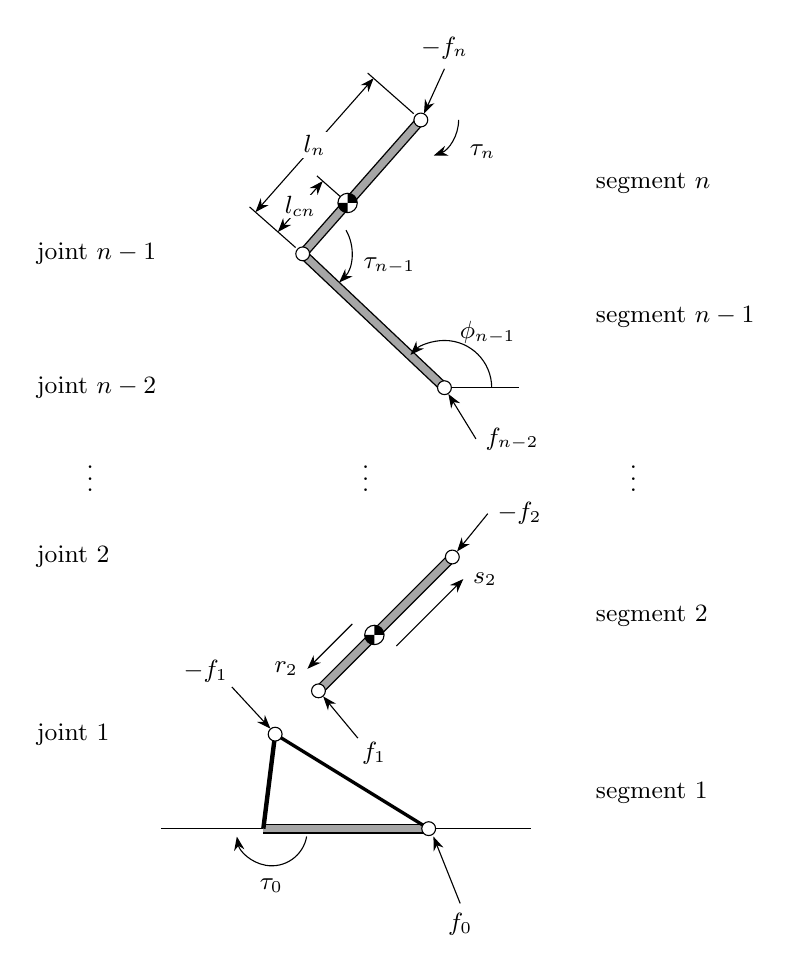
\begin{tikzpicture}[>={Stealth[length=5pt]}, font=\small,
  seg/.style={draw=black, double=black!35, double distance=2.6pt,
    line width=0.5pt},
  joint/.style={circle, draw, fill=white, inner sep=0pt, minimum size=5pt}]
  \newcommand{\com}[1]{%
    \fill[white] (#1) circle (3.5pt);
    \fill (#1) -- ++(3.5pt,0) arc[start angle=0, end angle=90, radius=3.5pt] -- cycle;
    \fill (#1) -- ++(-3.5pt,0) arc[start angle=180, end angle=270, radius=3.5pt] -- cycle;
    \draw (#1) circle (3.5pt);}
  % ground and segment 1 (foot)
  \draw (-0.4,0) -- (4.3,0);
  \coordinate (H) at (0.9,0); \coordinate (A) at (1.05,1.2);
  \coordinate (T) at (3.0,0);
  \draw[seg] (H) -- (T);
  \draw[line width=1.6pt] (H) -- (A);
  \draw[line width=1.2pt] (A) -- (T);
  \draw[->] (1.45,-0.1) arc[start angle=-10, end angle=-170, radius=0.45];
  \node at (1.0,-0.72) {$\tau_0$};
  \draw[->] (3.4,-0.95) -- (3.06,-0.1) node[pos=0, below] {$f_0$};
  \draw[->] (0.5,1.8) -- (0.99,1.27) node[pos=0, above left=-2pt] {$-f_1$};
  % segment 2
  \coordinate (B2) at (1.6,1.75); \coordinate (J2) at (3.3,3.45);
  \coordinate (C2) at (2.31,2.46);
  \draw[seg] (B2) -- (J2);
  \draw[->] (2.03,2.60) -- (1.46,2.03) node[left] {$r_2$};
  \draw[->] (2.59,2.32) -- (3.44,3.17) node[right] {$s_2$};
  \draw[->] (2.1,1.15) -- (1.66,1.68) node[pos=0, below right=-2pt] {$f_1$};
  \draw[->] (3.75,4.0) -- (3.36,3.52) node[pos=0, right] {$-f_2$};
  \com{C2}
  \node[joint] at (A) {}; \node[joint] at (T) {};
  \node[joint] at (B2) {}; \node[joint] at (J2) {};
  % ellipses
  \node at (-1.3,4.55) {$\vdots$};
  \node at (2.2,4.55) {$\vdots$};
  \node at (5.6,4.55) {$\vdots$};
  % segment n-1
  \coordinate (Jn2) at (3.2,5.6); \coordinate (Jn1) at (1.4,7.3);
  \draw[seg] (Jn2) -- (Jn1);
  \draw (Jn2) -- ++(0.95,0);
  \draw[->] (3.8,5.6) arc[start angle=0, end angle=136, radius=0.6];
  \node at (3.75,6.3) {$\phi_{n-1}$};
  \draw[->] (3.6,4.95) -- (3.25,5.52) node[pos=0, right] {$f_{n-2}$};
  % segment n
  \coordinate (Tn) at (2.9,9.0); \coordinate (Cn) at (1.97,7.946);
  \draw[seg] (Jn1) -- (Tn);
  \draw[->] (1.95,7.6) arc[start angle=30, end angle=-45, radius=0.55];
  \node[right] at (2.05,7.15) {$\tau_{n-1}$};
  \draw[->] (3.38,9.0) arc[start angle=0, end angle=-70, radius=0.48];
  \node[right] at (3.4,8.6) {$\tau_n$};
  \draw[->] (3.2,9.65) -- (2.94,9.08) node[pos=0, above] {$-f_n$};
  % dimension lines l_n (outer) and l_cn (inner), offset normal to segment n
  \draw[thin] (1.31,7.38) -- (0.725,7.896);
  \draw[thin] (2.81,9.08) -- (2.225,9.596);
  \draw[thin] (1.88,8.025) -- (1.58,8.29);
  \draw[<->] (0.8,7.83) -- (2.3,9.53)
    node[midway, fill=white, inner sep=1pt] {$l_n$};
  \draw[<->] (1.085,7.578) -- (1.655,8.224)
    node[midway, fill=white, inner sep=0.5pt] {$l_{cn}$};
  \com{Cn}
  \node[joint] at (Jn2) {}; \node[joint] at (Jn1) {}; \node[joint] at (Tn) {};
  % column labels
  \foreach \y/\t in {1.2/1, 3.45/2, 5.6/n-2, 7.3/n-1}
    \node[anchor=west] at (-2.1,\y) {joint $\t$};
  \foreach \y/\t in {0.45/1, 2.7/2, 6.5/n-1, 8.2/n}
    \node[anchor=west] at (5.0,\y) {segment $\t$};
\end{tikzpicture}
\caption{Two-dimensional body segment model (redrawn from \cite{Kuo1998}).
The $n$ segments are connected by $n-1$ joints. At joint $i$, a joint torque
$\tau_i$ and an intersegmental reaction force $f_i$ act on the two adjacent
segments with opposite signs. Segment $i$ has orientation $\phi_i$, length
$l_i$, and center of mass at distance $l_{ci}$ from its proximal end;
$r_i$ and $s_i$ point from its center of mass to its joints. Arrows mark
points of application only, not directions. Joint torques are positive in
extension, and angles are measured counterclockwise from the horizontal.}
\label{fig:1}
\end{figure}

\paragraph{Proposed Least-Squares Method.} Instead of relaxing boundary
conditions, the method relaxes the measurements: it seeks the joint torques
that require the smallest adjustment of the measurements to make them
mutually consistent. This is a static optimization in matrix form, solved by
a pseudoinverse. The ground reaction forces and angular accelerations are the
measurements to be adjusted, and the joint torques are the estimated
variables. The intersegmental forces $f_i$, $i=2,\ldots,n$, need not be
estimated, because they do no work and can be recovered from the estimated
torques.

The first set of equations is the equations of motion relating joint torques
and angular accelerations,
\begin{equation}
M(\phi)\ddot{\phi} = Q\tau + g(\phi) + v(\phi,\dot{\phi})
\label{eq:3}
\end{equation}
where $M$ is the mass matrix, $Q$ converts joint torques to segment torques,
and $g$ and $v$ hold the gravitational and velocity-dependent terms
(Appendix~A). The second set is found by deriving the equations of motion
with additional degrees of freedom for segment 1, and solving for the
constraint forces that keep it motionless; these equal the ground reactions.
The result is linear in $\ddot{\phi}$,
\begin{equation}
C(\phi)\ddot{\phi} = \begin{bmatrix}\tau_0\\ f_0\end{bmatrix}
+ c(\phi,\dot{\phi})
\label{eq:4}
\end{equation}
where $C(\phi)$ relates angular accelerations to reaction forces
(Appendix~A). Substituting $\ddot{\phi}$ from (\ref{eq:3}) into (\ref{eq:4})
gives a relation linear in $\tau$:
\begin{equation}
C(\phi) M^{-1}(\phi) Q\tau
= \begin{bmatrix}\tau_0\\ f_0\end{bmatrix} + c(\phi,\dot{\phi})
- C(\phi) M^{-1}(\phi)\{g(\phi) + v(\phi,\dot{\phi})\}.
\label{eq:5}
\end{equation}
Combining (\ref{eq:3}) and (\ref{eq:5}) and substituting the measured ground
reactions and angular accelerations on the right-hand side gives the
overdetermined system\tnote{The original prints the lower block of the
left-hand matrix as $M^{-1}(\phi)$; from (\ref{eq:3}),
$\ddot{\phi}=M^{-1}(Q\tau+g+v)$, so it must be $M^{-1}(\phi) Q$. The
original also prints the identity in the last term, and below, as
$I^{n\times n}$; since $\phi$ and $\ddot{\phi}$ have $n-1$ entries, it is
$I^{(n-1)\times(n-1)}$. Finally, the original prints $c(\phi,\ddot{\phi})$ in
the definition of $b$ below; the argument is $\dot{\phi}$, as in
(\ref{eq:4}).}
\begin{subequations}
\begin{equation}
\begin{bmatrix}C(\phi) M^{-1}(\phi) Q\\ M^{-1}(\phi) Q
\end{bmatrix}\tau
= \begin{bmatrix}\tau_0'\\ f_0'\\ \ddot{\phi}'\end{bmatrix}
+ \begin{bmatrix}c(\phi,\dot{\phi})\\ 0\end{bmatrix}
- \begin{bmatrix}C(\phi)\\ I^{(n-1)\times(n-1)}\end{bmatrix}
M^{-1}(\phi)\{g(\phi) + v(\phi,\dot{\phi})\}.
\label{eq:6a}
\end{equation}
Defining
\[
A \equiv \begin{bmatrix}C(\phi) M^{-1}(\phi) Q\\
M^{-1}(\phi) Q\end{bmatrix},
\qquad
b \equiv \begin{bmatrix}\tau_0'\\ f_0'\\ \ddot{\phi}'\end{bmatrix}
+ \begin{bmatrix}c(\phi,\dot{\phi})\\ 0\end{bmatrix}
- \begin{bmatrix}C(\phi)\\ I^{(n-1)\times(n-1)}\end{bmatrix}
M^{-1}(\phi)\{g(\phi) + v(\phi,\dot{\phi})\},
\]
(\ref{eq:6a}) takes the form
\begin{equation}
A\tau = b,
\label{eq:6b}
\end{equation}
\end{subequations}
where $A$ and $b$ have more rows than $\tau$ by the number of ground reaction
measurements. With noisy measurements there is in general no exact solution,
and static optimization finds the torques that best agree with the
measurements in the least-squares sense,
\begin{equation}
\tau = \arg\min_{\tau}\|A\tau - b\|^2
\label{eq:7}
\end{equation}
where, for a vector of length $m$, $\|x\|^2\equiv(1/m)\sum_{j=1}^{m}x_j^2$.
The linear form of (\ref{eq:6b}) admits a pseudoinverse solution
\cite{Strang1988}; a stochastic formulation \cite{StarkWoods1986} also yields
a statistical description of the errors. Let the covariance of the
zero-mean measurement errors be
\[
E\left[\left(\begin{bmatrix}\tau_0'\\ f_0'\\ \ddot{\phi}'\end{bmatrix}
- \begin{bmatrix}\bar{\tau}_0\\ \bar{f}_0\\ \ddot{\bar{\phi}}\end{bmatrix}\right)
\left(\begin{bmatrix}\tau_0'\\ f_0'\\ \ddot{\phi}'\end{bmatrix}
- \begin{bmatrix}\bar{\tau}_0\\ \bar{f}_0\\ \ddot{\bar{\phi}}\end{bmatrix}\right)^T
\right] = W.
\]
If the errors are independent, $W$ is diagonal with the measurement
variances. The optimal estimate is
\begin{equation}
\tau = (A^T W^{-1} A)^{-1} A^T W^{-1} b
\label{eq:8}
\end{equation}
i.e., the weighted pseudoinverse of $A$ applied to the measurements. It is
the unbiased ($E[\tau]=\bar{\tau}$) linear estimator with minimum error
covariance $E[(\tau-\bar{\tau})(\tau-\bar{\tau})^T]$.

The estimate satisfies the boundary conditions exactly, and handles missing
measurements naturally: an unavailable or unreliable entry of $\ddot{\phi}'$,
$f_0'$, or $\tau_0'$ is removed by setting its variance in $W$ to infinity
(equivalently, its entry of $W^{-1}$ to zero), which is valid as long as the
remaining rows of (\ref{eq:8}) are well conditioned and of sufficient rank.
In practice, (\ref{eq:8}) is better solved by a method such as singular value
decomposition than by forming the pseudoinverse explicitly
\cite{GolubVanLoan1989}. If very poor measurements make the weighting
ill-conditioned, the condition number of the matrix multiplying $b$ in
(\ref{eq:8}) can be monitored and $W$ rescaled to keep it moderate (e.g.,
about 100); this is rarely needed.

\paragraph{Correction of Measurement Bias.} Constant measurement biases (for
example from load-cell drift, a wrong body-mass estimate, or misalignment
between force plate and motion capture) can be removed by including them as
estimation variables and estimating over all time steps at once. Let the
$n_b$ unknown biases form a vector $\beta$, and modify (\ref{eq:6b}) to
\begin{equation}
A[k]\tau[k] = b[k] + B\beta
\label{eq:9}
\end{equation}
where $[k]$ denotes evaluation at time step $k$, of $N$ in total. The
selection matrix $B$ is $n_m\times n_b$, where $n_m$ is the length of $b[k]$,
with $B_{ij}=1$ if bias $j$ acts on measurement $i$ and $B_{ij}=0$ otherwise.
Stacking all time steps gives the block linear system
\begin{equation}
\begin{bmatrix}
A[1] & & & & -B\\
& A[2] & & & -B\\
& & \ddots & & -B\\
& & & A[N] & -B
\end{bmatrix}
\begin{bmatrix}\tau[1]\\ \tau[2]\\ \vdots\\ \tau[N]\\ \beta\end{bmatrix}
= \begin{bmatrix}b[1]\\ b[2]\\ \vdots\\ b[N]\end{bmatrix}.
\label{eq:10}
\end{equation}
This system, of size $N n_m$ by $((n-1)N+n_b)$,\tnote{The original gives the
size as ``$n_m$ by $(n\cdot N+n_b)$''. The system has $N$ row blocks of
length $n_m$, and each $\tau[k]$ has $n-1$ entries.} is much larger than a
single $A[k]$, but it is sparse and can be solved efficiently with sparse
algorithms \cite{GolubVanLoan1989}.

\paragraph{Error Analysis.} For the conventional method, (\ref{eq:1}) and
(\ref{eq:2}) for all segments are assembled into a matrix equation of the
form (Appendix~A)
\begin{equation}
\tau = F\begin{bmatrix}\ddot{\phi}'\\ \tau_0'\\ f_0'\end{bmatrix}
+ \gamma.
\label{eq:11}
\end{equation}
The covariance of the Newton--Euler torque error is\tnote{In (\ref{eq:12}),
$W$ must be ordered to match the stacking
$[\ddot{\phi}'^T\ \tau_0'\ f_0'^T]^T$ of (\ref{eq:11}), which differs from
the stacking $[\tau_0'\ f_0'^T\ \ddot{\phi}'^T]^T$ used to define $W$ above;
permute the rows and columns of $W$ accordingly.}
\begin{equation}
X_{NE} = F W F^T.
\label{eq:12}
\end{equation}
For the least-squares method,\tnote{The original defines
$A^{\#}\equiv(A^TA)^{-1}A^T$, for which the second equality in
(\ref{eq:13}) does not hold unless $W$ is a multiple of the identity. The
equality holds for the weighted pseudoinverse used in (\ref{eq:8}), given
here.}
\begin{equation}
X_{LS} = (A^TW^{-1}A)^{-1} = A^{\#}WA^{\#T}
\label{eq:13}
\end{equation}
where $A^{\#}\equiv(A^TW^{-1}A)^{-1}A^TW^{-1}$ is the weighted pseudoinverse
of $A$. The predicted joint torque error variances are the diagonal elements
of $X_{LS}$. With zero-mean measurement noise, both methods give zero-mean
torque errors.

\paragraph{``Experimental'' Comparison of Methods.} A simulation with known
torques was used to compare the methods and to test the error predictions.
The benchmark is postural sway of a four-segment body in the sagittal plane
(model and parameters in Appendix~A). Ground reaction forces (horizontal and
vertical) and torque, and the positions of markers at the joint centers, were
computed and corrupted with zero-mean white noise of known variance, sampled
at \SI{60}{\hertz}, and low-pass filtered (third-order Butterworth,
\SI{5}{\hertz} cutoff, forward and backward passes). First and second
derivatives of the angles were found by second-order finite differences. The
motion lasted \SI{4}{\second}, about the ankle, knee, and hip, and was driven
by feedforward joint torques made of sinusoids from \SI{0.5}{\hertz} to
\SI{2.2}{\hertz} with random phases plus a stabilizing feedback component
(Fig.~\ref{fig:2}). The measurement noise covariance was computed for each
case and used in (\ref{eq:8}). Four sets of simulations were run.
\begin{enumerate}
\item \emph{Error prediction.} Fifty ensembles with force noise
\SI{0.1}{\newton} (\SI{0.1}{\newton\metre} for torque) and marker noise
\SI{1}{\centi\metre} (horizontal and vertical). The square root of the
ensemble-averaged square error over time was compared with the square roots
of the diagonals of the predicted covariance.
\item \emph{Noise levels.} Force noise standard deviations from
\SI{0.001}{\newton} (\SI{0.001}{\newton\metre}) to \SI{10}{\newton}
(\SI{1}{\newton\metre}) in increments of a factor of 10, and marker noise from
\SI{0.01}{\centi\metre} to \SI{3.2}{\centi\metre}, as stated in the original;
one ensemble per combination. Errors were summarized by the root
time-averaged square error of each joint,\tnote{The original prints the
summand of (\ref{eq:14}) with an unbalanced parenthesis,
$(\tau_i[k]-(\bar{\tau}_i[k])^2$.}
\begin{equation}
\mathrm{RMSE}i = \sqrt{\frac{1}{N}\sum_{k=1}^{N}
(\tau_i[k] - \bar{\tau}_i[k])^2}
\label{eq:14}
\end{equation}
and over all joints by the magnitude of the torque error vector,
\begin{equation}
\mathrm{RMSE} = \sqrt{\frac{1}{N}\sum_{k=1}^{N}\|\tau[k] - \bar{\tau}[k]\|^2}.
\label{eq:15}
\end{equation}
\item \emph{Missing measurements.} The noise of set 1, for every possible
combination of missing force-plate channels, one ensemble each.
\item \emph{Bias.} Misalignment of the force-plate and motion-capture
coordinate systems from \SI{0}{\centi\metre} to \SI{1}{\centi\metre} in steps
of \SI{0.1}{\centi\metre}, with the noise of set 1, one ensemble each.
\end{enumerate}

\begin{figure}[t]
\centering
\framebox{\parbox{0.8\textwidth}{\centering\vspace{1.5em}
Figure 2 is not reproduced here; see Fig.~2 of \cite{Kuo1998}.\vspace{1.5em}}}
\caption{Benchmark simulation of postural movement: (a) ankle, knee, and hip
angles; (b) joint torques; (c) ground reaction data (horizontal force $F_x$,
vertical force $F_y$, torque $T$), all versus time.}
\label{fig:2}
\end{figure}

\section*{Results}

For the noise of set 1, Newton--Euler was more precise at the ankle and knee:
ankle RMSE1 \SI{0.043}{\newton\metre} versus \SI{0.61}{\newton\metre} for
least squares, knee RMSE2 \SI{1.43}{\newton\metre} versus
\SI{2.13}{\newton\metre}. At the hip it was much worse,
\SI{5.49}{\newton\metre} versus \SI{3.02}{\newton\metre} (RMSE3), so that the
overall least-squares RMSE was 34 percent lower (\SI{2.16}{\newton\metre}
versus \SI{3.27}{\newton\metre}); Newton--Euler also left a residual torque of
\SI{51.3}{\newton\metre} (RMSE4), and counting it would raise the reduction to
about 95 percent. Overall angular acceleration error fell by 30 percent, from
\SI{3.72}{\radian\per\second\squared} to \SI{2.60}{\radian\per\second\squared}
(Fig.~\ref{fig:3}).

The ensemble-averaged standard errors over time agree with the predictions of
(\ref{eq:12}) and (\ref{eq:13}) in trend: least squares outperforms
Newton--Euler, especially at the joint most distal to the force plate, where
about a 30 percent reduction is predicted. The predictions underestimate the
actual error (Fig.~\ref{fig:4}a,b); recomputing with exact angles and angular
velocities ($\phi'=\bar{\phi}$, $\dot{\phi}'=\dot{\bar{\phi}}$) brings actual
and predicted errors much closer (Fig.~\ref{fig:4}c), confirming that errors in
those quantities, which the model neglects, cause the underestimate.

Across noise levels (Fig.~\ref{fig:5}), error grows with both marker and force
noise for both methods, but least squares was more precise in every case,
with a relative RMSE reduction of 20 to 60 percent for 48 of the 56
combinations and a median of about 35 percent. With missing force
measurements (Fig.~\ref{fig:6}), least squares was more precise whenever at
least one force-plate channel was available; with only accelerations the
system is determinate and the two methods coincide. The largest reductions
were with horizontal force and torque (91 percent), horizontal and vertical
force (78 percent), torque alone (90 percent), and horizontal force alone
(76 percent). With misalignment bias and all force channels
(Fig.~\ref{fig:7}), Newton--Euler RMSE grew linearly, from
\SI{3.27}{\newton\metre} to \SI{7.52}{\newton\metre} at \SI{1}{\centi\metre}
(a factor of 2.3), while the bias-corrected least-squares estimate stayed at
\SI{2.17}{\newton\metre}; the relative reduction grew from 34 to 71 percent.

\begin{figure}[p]
\centering
\framebox{\parbox{0.8\textwidth}{\centering\vspace{1.5em}
Figure 3 is not reproduced here; see Fig.~3 of \cite{Kuo1998}.\vspace{1.5em}}}
\caption{Benchmark comparison of Newton--Euler and least squares: (a) joint
torque estimates versus actual torques at ankle, knee, and hip over time;
(b) time-averaged joint torque error for each joint and overall (RMSE);
(c) time-averaged joint angular acceleration error. Least squares lowers the
overall torque error and the acceleration error at every joint.}
\label{fig:3}
\vspace{1.5em}
\framebox{\parbox{0.8\textwidth}{\centering\vspace{1.5em}
Figure 4 is not reproduced here; see Fig.~4 of \cite{Kuo1998}.\vspace{1.5em}}}
\caption{Ensemble-averaged standard errors over time for Newton--Euler (NE)
and least squares (LS), for ankle, knee, and hip: actual versus predicted
(a) joint torque errors and (b) angular acceleration errors; (c) joint torque
errors with exact angles and angular velocities but noisy accelerations, for
which predictions are much closer to the actual errors.}
\label{fig:4}
\vspace{1.5em}
\framebox{\parbox{0.8\textwidth}{\centering\vspace{1.5em}
Figure 5 is not reproduced here; see Fig.~5 of \cite{Kuo1998}.\vspace{1.5em}}}
\caption{Joint torque estimation error for varying force and marker noise:
(a) absolute RMSE for both methods; (b) least-squares RMSE as a fraction of
Newton--Euler RMSE.}
\label{fig:5}
\end{figure}

\begin{figure}[t]
\centering
\framebox{\parbox{0.8\textwidth}{\centering\vspace{1.5em}
Figure 6 is not reproduced here; see Fig.~6 of \cite{Kuo1998}.\vspace{1.5em}}}
\caption{Joint torque RMSE for both methods for every combination of
available force-plate channels ($F_x$ horizontal force, $F_y$ vertical force,
$T$ torque), with all acceleration measurements used.}
\label{fig:6}
\vspace{1.5em}
\framebox{\parbox{0.8\textwidth}{\centering\vspace{1.5em}
Figure 7 is not reproduced here; see Fig.~7 of \cite{Kuo1998}.\vspace{1.5em}}}
\caption{Joint torque RMSE for both methods versus misalignment between
force-plate and motion-capture coordinate systems.}
\label{fig:7}
\end{figure}

\section*{Discussion}

Least squares gave lower overall torque error than Newton--Euler at every
noise level tested. Newton--Euler is often better at the joints nearest the
force plate, but at the cost of much larger errors at distal joints and
residual forces and torques at the top. Least squares also estimates angular
accelerations and ground reactions with minimum mean-square error.

The method requires the measurement covariances. They can be estimated
roughly from the filtered (and differentiated) data, or computed from
equipment precision and a model of the processing (Appendix~B), although skin
motion, plate vibration, and non-white or non-Gaussian noise are hard to
model. The method is robust to these errors: in the benchmark, changing one
covariance by 100 percent changed the torque error by only about 7 percent on
average, and with all covariances set equal, least squares still beat
Newton--Euler in all but two of the 54 noise combinations tested. Accurate
covariances matter more for predicting the error. (\ref{eq:12}) and
(\ref{eq:13}) predict it well when angles and angular velocities are precise,
and even when they are not, the predictions still capture how the error
changes over time and how much least squares can improve precision.

The formulation is robust to missing measurements: without horizontal ground
reaction force, its error was only 7 percent larger than Newton--Euler's with
all measurements. It can use any number of measurements, as long as they
make the problem determinate and enter linearly in the estimated variables;
accelerometers, for example, could improve estimates at joints far from the
force plate. Constant biases can be estimated as long as the data make the
problem determinate, which is easily satisfied with many time steps; this
reduces the need to align or zero the force-plate and motion-capture origins
carefully (their axes must still be parallel). With a sparse solver in MATLAB,
the bias formulation ran about 6 percent \emph{faster} than the standard
inverse dynamics.

Dynamic optimization \cite{ChaoRim1973} treats the equations of motion as
differential equations and constrains the torque trajectory over time, and so
can in principle be more precise; static optimization treats them as
algebraic equations at each instant but is far easier to solve. The main
drawback of the least-squares method is that it needs the multibody equations
of motion and the equations relating ground reactions to joint torques, which
are harder to derive than iterating Newton--Euler \cite{Greenwood1988}; they
can, however, be obtained symbolically or numerically from kinematic
constraints as in Appendix~A. Finally, the method improves \emph{precision}
only; systematic errors from filtering, marker placement, or body segment
parameters still limit \emph{accuracy}.

\section*{Acknowledgments}

The original work was supported in part by the Whitaker Foundation, NSF Grant
IBN-9511814, NIH Grant P60DC02072-03, and the Claude Pepper Older Americans
Independence Center at the University of Michigan.

\bibliographystyle{plain}
\bibliography{Kuo1998}

%======================================================================
\clearpage
\section*{Appendix A: Equations for Four-Segment Model}
\setcounter{equation}{0}
\renewcommand{\theequation}{A\arabic{equation}}

The equations of motion (\ref{eq:3}) and the ground reaction equation
(\ref{eq:4}) for the four-segment benchmark are derived from the Newton--Euler
equations and simple kinematics. The result is exactly equivalent to the
equations from Lagrange's \cite{Greenwood1988} or Kane's
\cite{KaneLevinson1985} methods, needs no algebraic reduction when computed
numerically, and extends to more segments or to three dimensions
(Appendix~C). It is convenient to first derive the equations of motion with
segment 1 free to rotate; this superset of the equations includes the extra
degree of freedom used to solve for the ground reaction torque. The stacked
angular orientations, joint torques, center-of-mass positions, and reaction
forces are\tnote{The original denotes the stacked torque vector by an italic
$T$ here and by a script $\mathcal{T}$ in (\ref{eq:A5}) onward; $\mathcal{T}$
is used throughout.}
\[
\Phi \equiv \begin{bmatrix}\phi_1\\ \phi_2\\ \vdots\\ \phi_n\end{bmatrix}
= \begin{bmatrix}\phi_1\\ \phi\end{bmatrix},
\qquad
\mathcal{T} \equiv \begin{bmatrix}\tau_0\\ \tau_1\\ \vdots\\ \tau_{n-1}
\end{bmatrix}
= \begin{bmatrix}\tau_0\\ \tau\end{bmatrix},
\qquad
x_c \equiv \begin{bmatrix}x_{c1}\\ x_{c2}\\ \vdots\\ x_{cn}\end{bmatrix},
\qquad
f \equiv \begin{bmatrix}f_0\\ f_1\\ \vdots\\ f_{n-1}\end{bmatrix}.
\]
The kinematic constraints express the center-of-mass positions as functions of
the generalized coordinates (the segment angles):\tnote{The original prints
the last row of (\ref{eq:A1}) as $l_1s_1+l_2s_2+l_3c_3+l_{c4}s_4$; the third
term is $l_3s_3$.}
\begin{equation}
x_c = \begin{bmatrix}
l_{c1}c_1\\
l_{c1}s_1\\
l_1c_1 + l_{c2}c_2\\
l_1s_1 + l_{c2}s_2\\
l_1c_1 + l_2c_2 + l_{c3}c_3\\
l_1s_1 + l_2s_2 + l_{c3}s_3\\
l_1c_1 + l_2c_2 + l_3c_3 + l_{c4}c_4\\
l_1s_1 + l_2s_2 + l_3s_3 + l_{c4}s_4
\end{bmatrix}
\label{eq:A1}
\end{equation}
where $s_i\equiv\sin\phi_i$, $c_i\equiv\cos\phi_i$, $l_i$ is the length of
segment $i$, and $l_{ci}$ is the distance from the end of segment $i$ nearest
the ground to its center of mass (Fig.~\ref{fig:1}). The first and second time
derivatives of (\ref{eq:A1}) are written with the Jacobian and its
derivative,\tnote{The original prints the $(1,1)$ entry of $J$ as
$-l_{c0}s_0$; it is $-l_{c1}s_1$.}
\[
J \equiv \frac{\partial x_c}{\partial\Phi}, \qquad
J = \begin{bmatrix}
-l_{c1}s_1 & 0 & 0 & 0\\
l_{c1}c_1 & 0 & 0 & 0\\
-l_1s_1 & -l_{c2}s_2 & 0 & 0\\
l_1c_1 & l_{c2}c_2 & 0 & 0\\
-l_1s_1 & -l_2s_2 & -l_{c3}s_3 & 0\\
l_1c_1 & l_2c_2 & l_{c3}c_3 & 0\\
-l_1s_1 & -l_2s_2 & -l_3s_3 & -l_{c4}s_4\\
l_1c_1 & l_2c_2 & l_3c_3 & l_{c4}c_4
\end{bmatrix},
\]
\[
\dot{J} = \begin{bmatrix}
-l_{c1}c_1\dot{\phi}_1 & 0 & 0 & 0\\
-l_{c1}s_1\dot{\phi}_1 & 0 & 0 & 0\\
-l_1c_1\dot{\phi}_1 & -l_{c2}c_2\dot{\phi}_2 & 0 & 0\\
-l_1s_1\dot{\phi}_1 & -l_{c2}s_2\dot{\phi}_2 & 0 & 0\\
-l_1c_1\dot{\phi}_1 & -l_2c_2\dot{\phi}_2 & -l_{c3}c_3\dot{\phi}_3 & 0\\
-l_1s_1\dot{\phi}_1 & -l_2s_2\dot{\phi}_2 & -l_{c3}s_3\dot{\phi}_3 & 0\\
-l_1c_1\dot{\phi}_1 & -l_2c_2\dot{\phi}_2 & -l_3c_3\dot{\phi}_3
& -l_{c4}c_4\dot{\phi}_4\\
-l_1s_1\dot{\phi}_1 & -l_2s_2\dot{\phi}_2 & -l_3s_3\dot{\phi}_3
& -l_{c4}s_4\dot{\phi}_4
\end{bmatrix}
\]
so that
\begin{align}
\dot{x}_c &= J\dot{\Phi} \label{eq:A2}\\
\ddot{x}_c &= J\ddot{\Phi} + \dot{J}\dot{\Phi}. \label{eq:A3}
\end{align}
Summing the forces on each segment, Newton's equation is
\begin{equation}
S_2 f = M_D\ddot{x}_c + g_V
\label{eq:A4}
\end{equation}
where
\[
S_2 \equiv \begin{bmatrix}
I^{2\times2} & -I^{2\times2} & & \\
& I^{2\times2} & -I^{2\times2} & \\
& & I^{2\times2} & -I^{2\times2}\\
& & & I^{2\times2}
\end{bmatrix},
\qquad
\begin{aligned}
M_D &\equiv \operatorname{diag}(m_1, m_1, m_2, m_2, m_3, m_3, m_4, m_4)\\
g_V &\equiv \begin{bmatrix}0 & m_1 & 0 & m_2 & 0 & m_3 & 0 & m_4
\end{bmatrix}^T g
\end{aligned}
\]
with $I^{2\times2}$ the $2\times2$ identity and $g$ the gravitational
constant. Euler's equation is
\begin{equation}
I\ddot{\Phi} = S_1\mathcal{T} + P f
\label{eq:A5}
\end{equation}
where $I\equiv\operatorname{diag}(I_1,I_2,I_3,I_4)$ is the diagonal matrix of
segment moments of inertia, and
\[
S_1 \equiv \begin{bmatrix}
1 & -1 & & \\
& 1 & -1 & \\
& & 1 & -1\\
& & & 1
\end{bmatrix},
\]
{\footnotesize\setlength{\arraycolsep}{2.5pt}
\[
P \equiv \begin{bmatrix}
l_{c1}s_1 & -l_{c1}c_1 & (l_1-l_{c1})s_1 & -(l_1-l_{c1})c_1
& 0 & 0 & 0 & 0\\
0 & 0 & l_{c2}s_2 & -l_{c2}c_2
& (l_2-l_{c2})s_2 & -(l_2-l_{c2})c_2 & 0 & 0\\
0 & 0 & 0 & 0 & l_{c3}s_3 & -l_{c3}c_3
& (l_3-l_{c3})s_3 & -(l_3-l_{c3})c_3\\
0 & 0 & 0 & 0 & 0 & 0 & l_{c4}s_4 & -l_{c4}c_4
\end{bmatrix}.
\]}
The forces $f$ are eliminated by substituting (\ref{eq:A3}) and (\ref{eq:A4})
into (\ref{eq:A5}):
\begin{equation}
I\ddot{\Phi} = S_1\mathcal{T}
+ P(S_2^{-1} M_D J\ddot{\Phi}
+ S_2^{-1} M_D\dot{J}\dot{\Phi} + S_2^{-1} g_V)
\label{eq:A6}
\end{equation}
which rearranges to
\begin{equation}
\mathcal{M}\ddot{\Phi} = S_1\mathcal{T} + \mathcal{V} + \mathcal{G}
\label{eq:A7}
\end{equation}
with
\[
\mathcal{M} \equiv I - P S_2^{-1} M_D J, \qquad
\mathcal{V} \equiv P S_2^{-1} M_D\dot{J}\dot{\Phi}, \qquad
\mathcal{G} \equiv P S_2^{-1} g_V.
\]
Equation (\ref{eq:A7}) partitions into an equation for the motionless segment
1 and the equations of motion (\ref{eq:3}) for the remaining
segments:\tnote{The original omits the ``$+$'' between the first two vectors
on the right-hand side of (\ref{eq:A8}), and calls the motionless segment
``segment 0''; it is segment 1, whose Euler equation is the first row. Here
$m_{ij}$ are entries of $\mathcal{M}$ (not masses). Reading off the lower
blocks: $M(\phi)$ is the lower-right $(n-1)\times(n-1)$ block of
$\mathcal{M}$; $g(\phi)$ and $v(\phi,\dot{\phi})$ are rows $2,\ldots,n$ of
$\mathcal{G}$ and $\mathcal{V}$; and $Q$ is the lower-right block of $S_1$,
i.e., ones on the diagonal and $-1$ on the superdiagonal, so that
$Q\tau=[\tau_1-\tau_2\ \ \tau_2-\tau_3\ \ \cdots\ \ \tau_{n-1}]^T$.}
\begin{equation}
\begin{bmatrix}
m_{11} & m_{12}\ \ m_{13}\ \ m_{14}\\
\begin{matrix}m_{12}\\ m_{13}\\ m_{14}\end{matrix} & M(\phi)
\end{bmatrix}
\begin{bmatrix}0\\ \ddot{\phi}\end{bmatrix}
= \begin{bmatrix}\tau_0 - \tau_1\\ Q\tau\end{bmatrix}
+ \begin{bmatrix}\mathcal{V}_1\\ v(\phi,\dot{\phi})\end{bmatrix}
+ \begin{bmatrix}\mathcal{G}_1\\ g(\phi)\end{bmatrix}.
\label{eq:A8}
\end{equation}
The ground reaction forces follow from (\ref{eq:A4}),\tnote{The original
prints $\ddot{x}$ for $\ddot{x}_c$ in (\ref{eq:A9}).}
\begin{equation}
f_0 = S_2' M_D\ddot{x}_c + S_2' g_V
\label{eq:A9}
\end{equation}
where $S_2'\equiv[I^{2\times2}\ I^{2\times2}\ I^{2\times2}\ I^{2\times2}]$ is
the first (block) row of $S_2^{-1}$. Similarly, the ground reaction torque
follows from (\ref{eq:A7}),\tnote{The original prints (\ref{eq:A10}) as
$\tau_0=S_1'\mathcal{M}\ddot{\Phi}-\mathcal{V}_1-\mathcal{G}_1$. Solving
(\ref{eq:A7}) for $\mathcal{T}=S_1^{-1}(\mathcal{M}\ddot{\Phi}-\mathcal{V}
-\mathcal{G})$ and taking its first row gives the form shown, which was
verified numerically; the printed form is not equivalent.}
\begin{equation}
\tau_0 = S_1'(\mathcal{M}\ddot{\Phi} - \mathcal{V} - \mathcal{G})
\label{eq:A10}
\end{equation}
where $S_1'=[1\ 1\ 1\ 1]$ is the first row of $S_1^{-1}$. The following
definitions then yield (\ref{eq:4}):\tnote{The original prints the upper
entry of $c$ as $V_1+G_1$ and the lower entry as
$-S_2'M_D\dot{J}\dot{\Phi}+S_2'g_V$. Both are corrected to be consistent with
(\ref{eq:A3}), (\ref{eq:A9}), and (\ref{eq:A10}), and were verified
numerically. Also, $C(\phi)$ as defined multiplies $\ddot{\Phi}=[0\
\ddot{\phi}^T]^T$; in (\ref{eq:4}), where it multiplies $\ddot{\phi}$, its
first column (which multiplies $\ddot{\phi}_1=0$) is dropped.}
\[
C(\phi) \equiv \begin{bmatrix}S_1'\mathcal{M}\\
S_2' M_D J\end{bmatrix},
\qquad
c(\phi,\dot{\phi}) \equiv \begin{bmatrix}
S_1'(\mathcal{V} + \mathcal{G})\\
-S_2'M_D\dot{J}\dot{\Phi} - S_2'g_V
\end{bmatrix}.
\]

The same equations give the matrix $F$ of (\ref{eq:11}) and (\ref{eq:12})
with a few changes: (\ref{eq:A4}) and (\ref{eq:A5}) are rewritten to separate
the ground reaction measurements $f_0$ and $\tau_0$, and an extra degree of
freedom is added for the residual $\tau_n$, using
\[
\hat{\mathcal{T}} \equiv \begin{bmatrix}\tau_1\\ \tau_2\\ \vdots\\ \tau_n
\end{bmatrix},
\qquad
\hat{f} \equiv \begin{bmatrix}f_1\\ f_2\\ \vdots\\ f_n\end{bmatrix},
\qquad
\hat{S}_1 \equiv \begin{bmatrix}
-1 & & & \\
1 & -1 & & \\
& 1 & -1 & \\
& & 1 & -1
\end{bmatrix},
\]
\[
\hat{S}_2 \equiv \begin{bmatrix}
-I^{2\times2} & & & \\
I^{2\times2} & -I^{2\times2} & & \\
& I^{2\times2} & -I^{2\times2} & \\
& & I^{2\times2} & -I^{2\times2}
\end{bmatrix},
\qquad
P_0 \equiv \begin{bmatrix}
l_{c1}s_1 & -l_{c1}c_1\\
0 & 0\\
0 & 0\\
0 & 0
\end{bmatrix},
\]
{\footnotesize\setlength{\arraycolsep}{2.5pt}
\[
\hat{P} \equiv \begin{bmatrix}
(l_1-l_{c1})s_1 & -(l_1-l_{c1})c_1 & 0 & 0 & 0 & 0 & 0 & 0\\
l_{c2}s_2 & -l_{c2}c_2 & (l_2-l_{c2})s_2 & -(l_2-l_{c2})c_2
& 0 & 0 & 0 & 0\\
0 & 0 & l_{c3}s_3 & -l_{c3}c_3
& (l_3-l_{c3})s_3 & -(l_3-l_{c3})c_3 & 0 & 0\\
0 & 0 & 0 & 0 & l_{c4}s_4 & -l_{c4}c_4
& (l_4-l_{c4})s_4 & -(l_4-l_{c4})c_4
\end{bmatrix}
\]}
which rearrange (\ref{eq:A4}) and (\ref{eq:A5}) into\tnote{The original
prints the last term of (\ref{eq:A11}) as $-(S_2')^Tf_0$. Since
$\hat{S}_2^{-1}$ applied to $[I^{2\times2}\ 0\ 0\ 0]^T$ equals $-(S_2')^T$,
the sign is $+$, as in the analogous term of (\ref{eq:A12}); e.g., the first
block row gives $f_1=f_0-m_1(\ddot{x}_{c1}+[0\ 1]^Tg)$. Verified
numerically.}
\begin{align}
\hat{f} &= \hat{S}_2^{-1}\{M_D\ddot{x}_c + g_V\} + (S_2')^Tf_0
\label{eq:A11}\\
\hat{\mathcal{T}} &= \hat{S}_1^{-1}\{I\ddot{\Phi} - \hat{P}\hat{f}
- P_0 f_0\} + (S_1')^T\tau_0. \label{eq:A12}
\end{align}
The Newton--Euler output, $\hat{\mathcal{T}}$,\tnote{The original prints
$\mathcal{T}'$ here; the quantity computed in (\ref{eq:A13}) is
$\hat{\mathcal{T}}$.} is found by combining (\ref{eq:A3}), (\ref{eq:A11}),
and (\ref{eq:A12}):\tnote{The original prints the $f_0$ term of
(\ref{eq:A13}) as $+\{\hat{P}(S_2')^T-P_0\}f_0$, and correspondingly the
third block of the first matrix in (\ref{eq:A14}) as
$\hat{S}_1^{-1}\{\hat{P}(S_2')^T-P_0\}$. These follow from the sign
error in (\ref{eq:A11}); the corrected forms shown were verified
numerically.}
\begin{equation}
\hat{\mathcal{T}} = \hat{S}_1^{-1}\big\{I\ddot{\Phi}
- \hat{P}\hat{S}_2^{-1}\{M_D(J\ddot{\Phi} + \dot{J}\dot{\Phi})
+ g_V\} - \{\hat{P}(S_2')^T + P_0\}f_0\big\} + (S_1')^T\tau_0
\label{eq:A13}
\end{equation}
so that
\begin{equation}
\hat{\mathcal{T}} = \begin{bmatrix}
\hat{S}_1^{-1}(I - \hat{P}\hat{S}_2^{-1}M_DJ) (S_1')^T -\hat{S}_1^{-1}\{\hat{P}(S_2')^T + P_0\}
\end{bmatrix}
\begin{bmatrix}\ddot{\Phi}\\ \tau_0\\ f_0\end{bmatrix}
- \hat{S}_1^{-1}\hat{P}\hat{S}_2^{-1}(M_D\dot{J}\dot{\Phi} + g_V).
\label{eq:A14}
\end{equation}
Equation (\ref{eq:11}) follows by substituting the measured quantities into
(\ref{eq:A14}): $F$ is the first block matrix above with its first column
removed, because $\ddot{\phi}_1=0$,\tnote{The original says ``with the first
row removed''. The first \emph{column} multiplies $\ddot{\phi}_1=0$; all $n$
rows are kept, the last being the residual $\tau_n$.} and $\gamma$ is the
last term.

For completeness, the equations of motion (\ref{eq:A8}) are given explicitly
by the constants
\begin{align*}
b_1 &\equiv m_1l_{c1} + (m_2+m_3+m_4)l_1 &
b_2 &\equiv m_2l_{c2} + (m_3+m_4)l_2\\
b_3 &\equiv m_3l_{c3} + m_4l_3 &
b_4 &\equiv m_4l_{c4}\\[4pt]
a_{11} &\equiv I_1 + m_1l_{c1}^2 + (m_2+m_3+m_4)l_1^2 &
a_{22} &\equiv I_2 + m_2l_{c2}^2 + (m_3+m_4)l_2^2\\
a_{12} &\equiv b_2l_1 & a_{23} &\equiv b_3l_2\\
a_{13} &\equiv b_3l_1 & a_{24} &\equiv b_4l_2\\
a_{14} &\equiv b_4l_1 & a_{33} &\equiv I_3 + m_3l_{c3}^2 + m_4l_3^2\\
& & a_{34} &\equiv b_4l_3\\
& & a_{44} &\equiv I_4 + m_4l_{c4}^2
\end{align*}
which are used in the terms of (\ref{eq:A7}),\tnote{The original does not
define $c_{ij}$ and $s_{ij}$; the definitions given are the ones for which
these expressions equal $\mathcal{M}$, $\mathcal{V}$, and $\mathcal{G}$ as
defined after (\ref{eq:A7}), verified numerically. The original also prints
the $(2,3)$ entry of the matrix in $\mathcal{V}$ as $-a_{23}c_{23}\dot{\phi}_3$;
it is $-a_{23}s_{23}\dot{\phi}_3$.} with
$c_{ij}\equiv\cos(\phi_i-\phi_j)$ and $s_{ij}\equiv\sin(\phi_i-\phi_j)$:
\[
\mathcal{M}(\Phi) = \begin{bmatrix}
a_{11} & a_{12}c_{12} & a_{13}c_{13} & a_{14}c_{14}\\
a_{12}c_{12} & a_{22} & a_{23}c_{23} & a_{24}c_{24}\\
a_{13}c_{13} & a_{23}c_{23} & a_{33} & a_{34}c_{34}\\
a_{14}c_{14} & a_{24}c_{24} & a_{34}c_{34} & a_{44}
\end{bmatrix},
\]
\[
\mathcal{V}(\Phi,\dot{\Phi}) = \begin{bmatrix}
0 & -a_{12}s_{12}\dot{\phi}_2 & -a_{13}s_{13}\dot{\phi}_3
& -a_{14}s_{14}\dot{\phi}_4\\
a_{12}s_{12}\dot{\phi}_1 & 0 & -a_{23}s_{23}\dot{\phi}_3
& -a_{24}s_{24}\dot{\phi}_4\\
a_{13}s_{13}\dot{\phi}_1 & a_{23}s_{23}\dot{\phi}_2 & 0
& -a_{34}s_{34}\dot{\phi}_4\\
a_{14}s_{14}\dot{\phi}_1 & a_{24}s_{24}\dot{\phi}_2
& a_{34}s_{34}\dot{\phi}_3 & 0
\end{bmatrix}
\begin{bmatrix}\dot{\phi}_1\\ \dot{\phi}_2\\ \dot{\phi}_3\\ \dot{\phi}_4
\end{bmatrix},
\]
\[
\mathcal{G}(\Phi) = \begin{bmatrix}-b_1c_1 & -b_2c_2 & -b_3c_3 & -b_4c_4
\end{bmatrix}^T g.
\]
The benchmark parameter values are
\[
\begin{aligned}
l_1 &= \SI{0.177}{\metre}, & l_2 &= \SI{0.405}{\metre}, &
l_3 &= \SI{0.440}{\metre}, & l_4 &= \SI{0.795}{\metre},\\
l_{c1} &= \SI{0.086}{\metre}, & l_{c2} &= \SI{0.235}{\metre}, &
l_{c3} &= \SI{0.268}{\metre}, & l_{c4} &= \SI{0.302}{\metre},\\
m_1 &= \SI{1.78}{\kilogram}, & m_2 &= \SI{7.30}{\kilogram}, &
m_3 &= \SI{15.5}{\kilogram}, & m_4 &= \SI{44.6}{\kilogram},\\
I_1 &= \SI{0.0080}{\kilogram\metre\squared}, &
I_2 &= \SI{0.097}{\kilogram\metre\squared}, &
I_3 &= \SI{0.253}{\kilogram\metre\squared}, &
I_4 &= \SI{1.51}{\kilogram\metre\squared}.
\end{aligned}
\]

%======================================================================
\section*{Appendix B: Prediction of Measurement Noise Covariance}
\setcounter{equation}{0}
\renewcommand{\theequation}{B\arabic{equation}}

Noise propagation through angle extraction, filtering, and numerical
differentiation can be estimated by modeling each process as an affine
operation on noisy measurements,
\begin{equation}
y = Zx + z
\label{eq:B1}
\end{equation}
where the estimates $y$ are linear in the measurements $x$ plus a constant
$z$. With additive white noise $w$ of zero mean and covariance $W$,
$x=\bar{x}+w$, the error in $y$ has zero mean and covariance
\begin{equation}
E[(y-\bar{y})(y-\bar{y})^T] = ZWZ^T.
\label{eq:B2}
\end{equation}

\paragraph{Error Covariance From Extraction of Angular Orientation From
Marker Positions.} With markers at the joint centers, the orientation of each
segment is
\begin{equation}
\phi_i = \tan^{-1}\frac{y_i - y_{i-1}}{x_i - x_{i-1}}
\label{eq:B3}
\end{equation}
where $x_i$ and $y_i$ are the horizontal and vertical marker positions at
joint $i$. Taking partial derivatives of (\ref{eq:B3}), the error covariance
of $\phi$ is\tnote{The original prints the diagonal entries of (\ref{eq:B4})
as $2/l_i$, which is dimensionally inconsistent with $W_x$ in
\si{\metre\squared} and $W_{\phi}$ in \si{\radian\squared}. Linearizing
(\ref{eq:B3}) with two independent markers per segment gives $2/l_i^2$. (The
diagonal form also neglects the correlation between adjacent segment angles
that share a marker.)}
\begin{equation}
W_{\phi} = E[(\phi-\bar{\phi})(\phi-\bar{\phi})^T]
= \begin{bmatrix}
2/l_2^2 & & & \\
& 2/l_3^2 & & \\
& & \ddots & \\
& & & 2/l_n^2
\end{bmatrix} W_x
\label{eq:B4}
\end{equation}
where $l_i$ is the length of segment $i$ and $W_x$ is the scalar variance of
marker position.

\paragraph{Error Covariance Due to Digital Filtering.} If the filter does
not appreciably degrade the signal, the filter-induced error variance is the
output variance of the filter driven by noise alone. A scalar white noise
sequence $w$ with zero mean and variance $W$ has autocorrelation
$R_{ww}[n]=W\cdot\delta[n]$ and power spectrum $S_{ww}(e^{j\omega})=W$. The
output of a filter with transfer function $H$ driven by this noise has
spectrum $S_{w_fw_f}=S_{ww}(e^{j\omega})|H(e^{j\omega})|^2$, and its variance
is the autocorrelation at lag 0 \cite{StarkWoods1986}:\tnote{The original
prints $R_{ww}[n]=W\cdot\delta[0]$ and writes the integrand of (\ref{eq:B5})
with $S_{xx}$; consistent with the surrounding definitions, these are
$\delta[n]$ and $S_{ww}$.}
\begin{equation}
W_f = R_{w_fw_f}[0] = \frac{1}{2\pi}\int_{-\pi}^{\pi}
S_{ww}(e^{j\omega})|H(e^{j\omega})|^2d\omega.
\label{eq:B5}
\end{equation}
Each channel is filtered independently, so the covariance is diagonal. The
integral is usually evaluated numerically, and underestimates the error if
the signal has significant content beyond the filter bandwidth.

\paragraph{Error Covariance Due to Numerical Differentiation.}
Differentiation adds a discretization error, which depends on the
approximation used, and amplifies measurement noise, which depends on the
noise covariance. For example, the three-point second derivative
is\tnote{The original writes $o(h^2)$ and describes it as ``other terms of
order $h^2$''; the standard notation for that is $\mathcal{O}(h^2)$.}
\begin{equation}
\ddot{\phi}[k] = \frac{1}{h^2}(\phi[k+1] - 2\phi[k] + \phi[k-1])
+ \mathcal{O}(h^2)
\label{eq:B6}
\end{equation}
where $h$ is the time step. With $\phi[k]=\bar{\phi}[k]+w_{\phi}[k]$, the error
covariance of $\ddot{\phi}$ is
\begin{equation}
\begin{split}
W_{\ddot{\phi}} &= E[(\ddot{\phi}-\ddot{\bar{\phi}})
(\ddot{\phi}-\ddot{\bar{\phi}})^T]\\
&= \frac{1}{h^4}\begin{bmatrix}1 & -2 & 1\end{bmatrix}
\begin{bmatrix}W_{\phi} & & \\ & W_{\phi} & \\ & & W_{\phi}\end{bmatrix}
\begin{bmatrix}1\\ -2\\ 1\end{bmatrix}\\
&= \frac{6}{h^4}W_{\phi}.
\end{split}
\label{eq:B7}
\end{equation}

\paragraph{Error Covariance Due to Combined Filtering and Numerical
Differentiation.} Filtering and differentiation both color the noise, so the
two estimates above cannot simply be chained. Instead, (\ref{eq:B5}) is
applied to a single transfer function $H(e^{j\omega})$ that combines the
low-pass filter and the numerical differentiation.

%======================================================================
\section*{Appendix C: Inverse Dynamics in Three Dimensions}
\setcounter{equation}{0}
\renewcommand{\theequation}{C\arabic{equation}}

In three dimensions the method is unchanged, but $f_i$, $\tau_i$, and $x_i$
become 3-vectors, and $\phi$ has as many entries as the system has degrees of
freedom (not necessarily three per joint). Segment angular velocity and
acceleration are functions of $\phi$, $\dot{\phi}$, and $\ddot{\phi}$ in a
suitable three-dimensional coordinate scheme. Deriving the body-centered
angular velocity $\omega_i$ and acceleration $\dot{\omega}_i$, Appendix~A
applies with the three-dimensional Euler equation
\begin{equation}
I_i\dot{\omega}_i + \omega_i\times I_i\omega_i
= r_i\times f_{i-1} - s_i\times f_i + \tau_{i-1} - \tau_i,
\label{eq:C1}
\end{equation}
where $I_i$ are $3\times3$ inertia tensors. The other matrices and vectors
are resized accordingly. In particular, $P$ becomes the block
matrix\tnote{The original prints the last diagonal block of $P$ as $r_n$; it
is the matrix $\hat{r}_n$.}
\[
P \equiv \begin{bmatrix}
\hat{r}_1 & -\hat{s}_1 & 0 & 0\\
0 & \hat{r}_2 & -\hat{s}_2 & 0\\
0 & 0 & \ddots & \vdots\\
0 & 0 & \cdots & \hat{r}_n
\end{bmatrix},
\qquad
\hat{z} \equiv \begin{bmatrix}
0 & -z_3 & z_2\\
z_3 & 0 & -z_1\\
-z_2 & z_1 & 0
\end{bmatrix},
\]
where $\hat{z}$ is the cross-product matrix of a vector $z$, so that $P f$
performs the cross products on the right-hand side of (\ref{eq:C1}). A
similar block matrix built from $\hat{\omega}_i$ is used on the left-hand
side.

\end{document}
